\pagebreak

\section{Misure}
Una volta studiato il funzionamento del fotomoltiplicatore, possiamo passare a prendere delle misure.\\

Fornendo al LED una tensione impulsata di 100 ns a circa 3.4 V è stato possibile osservare la rilevazione dei fotoni:

\begin{figure}[!h]
    \centering
    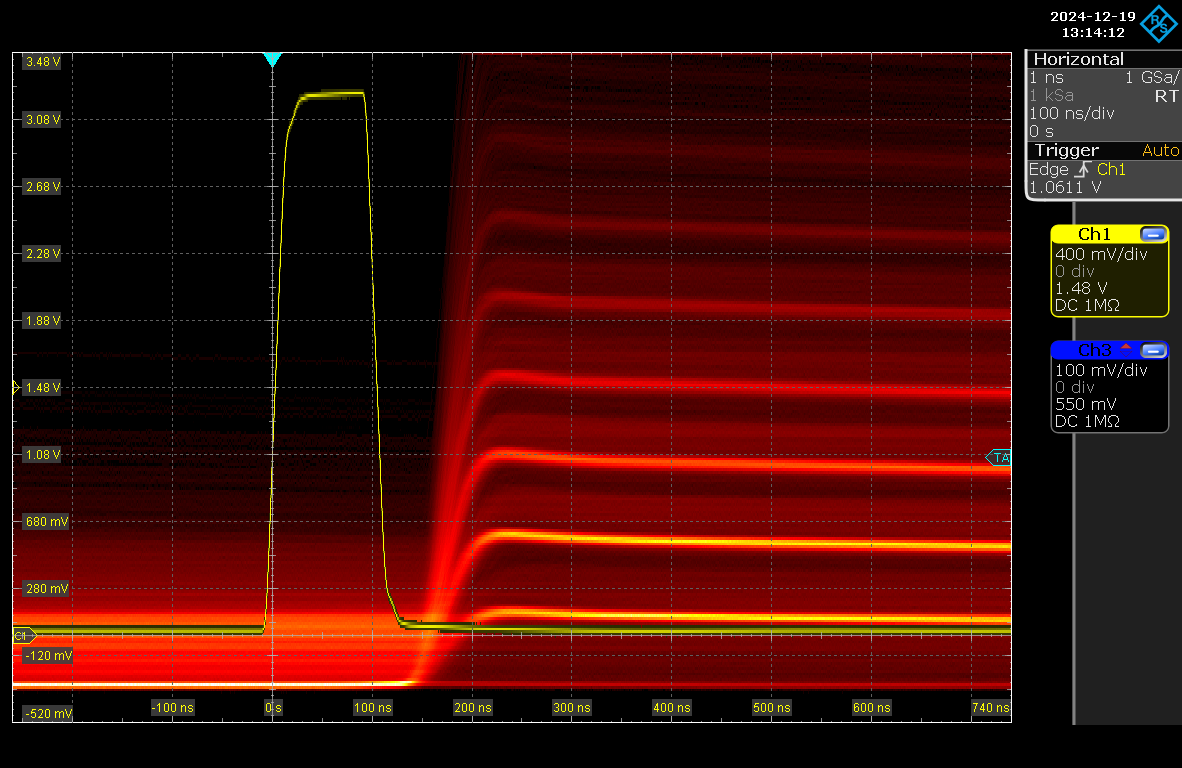
\includegraphics[width=0.5\linewidth]{Photomultiplier/assets/SiPm/SiPm.png}
    \caption{Prima visualizzazione dei segnali con persistance di 2 sec}
\end{figure}

E evidente la presenza di diverse zone con elevata densità di rilevazioni che corrispondono a un numero di fotoni crescente all'aumentare del voltaggio. Questo fenomeno è causato da 2 fotoni che arrivano in tempi molto ravvicinati e vengono rilevati come un unico evento.\\
Una volta collegato l'ADC e il comparatore all'uscita del Peak Hold, è stato possibile rilevare le onde:

\begin{figure}[!h]
    \centering
    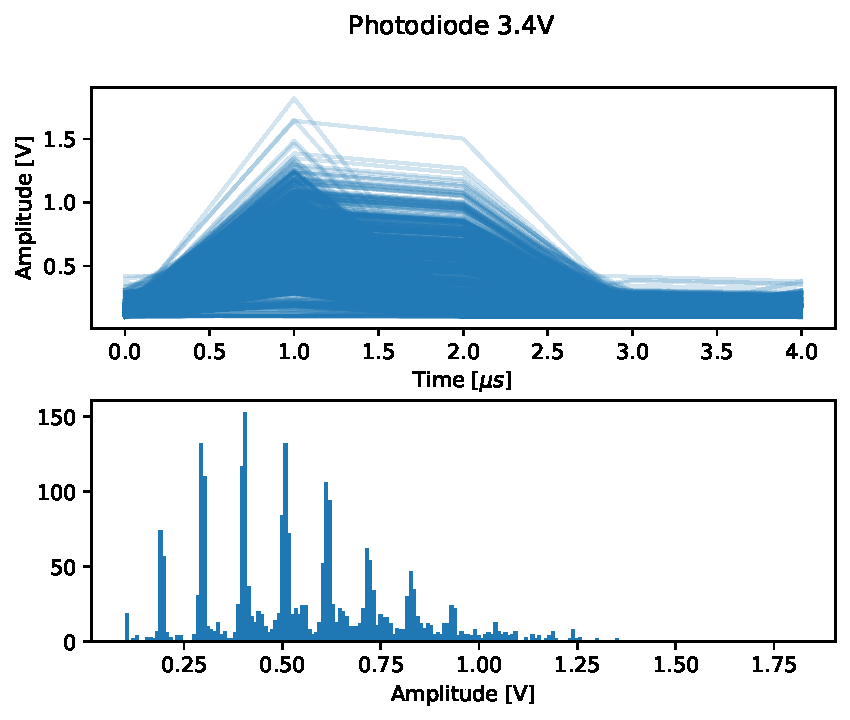
\includegraphics[width=0.5\linewidth]{Photomultiplier/assets/phot_3.4V.pdf}
    \caption{Segnale rilevato dall'ADC}
\end{figure}

Come si può notare, l'istogramma dei picchi è molto simile alla figura che si ha sull'oscilloscopio e i voltaggi sono molto simili.\\
Si può notare inoltre come i picchi siano quasi esattamente multipli 